\documentclass[11pt, oneside]{amsart}

\usepackage{amsmath}
\usepackage{amssymb}

%\usepackage{multibbl}
%\usepackage{bibtopic}

\usepackage{color}
\usepackage{dcolumn}
\usepackage{float}
\usepackage{graphicx}
%\usepackage{graphics}
\usepackage[latin9]{inputenc}
\usepackage{multirow}
\usepackage{rotating}
\usepackage{subfigure}
\usepackage{psfrag}
\usepackage{tabularx}
\usepackage[hyphens]{url}
\usepackage{wrapfig}

%\setcounter{secnumdepth}{3}
%\setcounter{tocdepth}{3}


\usepackage[bookmarks, bookmarksopen, bookmarksnumbered]{hyperref}
\usepackage[all]{hypcap}
\urlstyle{rm}

\definecolor{orange}{rgb}{1.0,0.3,0.0}
\definecolor{violet}{rgb}{0.75,0,1}
\definecolor{darkgreen}{rgb}{0,0.6,0}
\definecolor{cyan}{rgb}{0.2,0.7,0.7}
\definecolor{blueish}{rgb}{0.2,0.2,0.8}

\newcommand{\todo}[1]{{\color{blue}$\blacksquare$~\textsf{[TODO: #1]}}}
\newcommand{\huttonnote}[1]{ {\textcolor{magenta}    { ***Eric:      #1 }}}

% Don't use tt font for urls
\urlstyle{rm}

\begin{document}

\title[]{Building Sustainable Software - The CSDMS-2.0 Approach}

\author{
  Eric W. H. Hutton$^{\dag}$,
  Mark D. Piper$^{\dag}$,
  Albert J. Kettner$^{\dag}$,
  Irina Overeem$^{\dag}$}

\thanks{{}$^{\dag}$ Community Surface Dynamics Modeling System, Boulder, CO}

\begin{abstract}

Our abstract goes here.

\end{abstract}

\maketitle

\section{Building a User Community}


\section{The Community Surface Dynamics Modeling System}

The Community Surface Dynamics Modeling System (CSDMS)
~\cite{peckham2012component}
is an NSF-funded project that began in 2007. Its mission is to help a diverse
community of surface dynamics modelers and model users work together toward
common goals and standards. Part of this effort involves creating a repository
of open-source models. Another part involves converting models to plug-and-play
components that can be reused via dynamic linking within the CSDMS framework to
create new models. In building its modeling framework, CSDMS has leveraged
several existing, well-established and open-source software tools. For example,
CSDMS uses three tools from the Common Component Architecture (CCA) toolchain:
Babel, Bocca and Ccaffeine. Babel provides interoperability between components
written in different languages; it currently supports C, C++, Fortran, Java,
and Python. Bocca helps with creating CCA-compliant components and managing CCA
component projects. Ccaffeine is a CCA-compliant framework for linking
components into new applications. All three tools were designed to enable
component-based modeling in an HPC environment, but they can also be used on
desktop systems. CSDMS has developed innovative model/component interfaces for
use with the CCA tools, including the Basic Model Interface (BMI), which uses
the CSDMS Standard Names (both described below) and the framework-level
Component Model Interface (CMI). CSDMS has also developed a web-based client
for its modeling framework (the CSDMS Web Modeling Tool, WMT, described below)
that allows users to compose new models by connecting and configuring
components through a simple, browser-based graphical interface.

In order to realize the full power and benefits of component-based modeling, a
modeling framework like CSDMS needs an efficient mechanism to convert as many
open-source models as possible to reusable plug-and-play components. Since this
necessarily requires some involvement from each model's developer, this
mechanism must be designed to:

\begin{itemize}

\item require minimal effort from the model developer,

\item allow the model to continue to be used in a stand-alone manner,

\item not introduce new dependencies into the model,

\item not interfere with the developer's design,

\item not require any modeling framework-specific knowledge on the part of the
      developer,

\item not require the addition of new code which accommodates the needs of
      other models. 

\end{itemize}

These requirements became clear during the first few years of the CSDMS project
by working directly with model developers and listening to their concerns and
complaints about early designs and other frameworks.


\section{The Basic Modeling Interface}

The \emph{Basic Modeling Interface} (BMI) is a component-coupling library interface
specification designed by CSDMS~\cite{peckham2012component, syvitski2014plug}.
In this context, a component is software that models a particular environmental
process and can be "plugged into" another component. BMI addresses the
interaction of components that operate within a shared memory space by
providing entry points for: component control (initialize, run, and finalize
steps), data access, and metadata. This allows developers to write applications
that connect components to one another to form new models.

Most models require input variables and produce output variables. In a
component-based modeling framework, like CSDMS, a set of components becomes a
complete model when every component is able to obtain the input variables it
needs from another component. The CSDMS Standard Names were developed to
provide a practical solution to this semantic mediation problem
~\cite{peckham2012component, syvitski2014plug}.
While the CF Convention Standard Names, which were
introduced in the domain of the ocean and atmosphere model domains, have
somewhat overlapping goals, the CSDMS Standard Names provide a more
comprehensive set of naming rules and patterns for creating unique labels for
model variables that are not specific to any particular modeling domain.

CSDMS has found that BMI is an acceptable target for model developers. The use
of BMI has also dramatically reduced the effort required by CSDMS staff to
create and maintain components. There is now really just one universal CMI
wrapper to maintain that BMI-enabled models "plug into". The introduction of the
CSDMS Standard Names provides a practical and elegant solution to the semantic
mediation problem and Babel solves the language interoperability problem.
CSDMS has also assembled a large repository of surface process models that now
includes over 171 open-source models and 56 tools. The repository contains
terrestrial, coastal, marine, hydrological, carbonate and atmospheric models.
Geodynamic, atmospheric and ecosystem models will be added over the next few
years. So far, 55 of the 171 models have been wrapped for use as reusable
plug-and-play components (although only 6 are currently visible in the new WMT).
CSDMS has a steering committee, an executive committee, five working groups, six
focus research groups, an industrial consortium, and over 1150 members as of
June 2014. Members share information through a wiki.

The CSDMS Standard Names are a lingua franca for variable names between model
components. They play an important role in the BMI as they provide a mapping of
a model's internal variable names to a common language used by the BMI getter
and setter functions.


\section{CSDMS Standard Names}

The CSDMS Standard Names are currently being extended to solid Earth modeling
domains, including geodynamics, seismology, electromagnetic induction and
petrology, in the framework of the "Earth System Bridge" EarthCube project led
by PI Peckham. They also serve as the base for the metadata standard for
numerical models (MMF) which is currently in development within CSDMS.

We are acutely aware of multiple other efforts to provide cross-domain
ontologies in the realm of geosciences. PIs Peckham and Kelbert are involved
with the initial steps in semantic crosswalk development recently initialized
within the EarthCube community that aim to achieve synergy between these
currently divergent metadata ontologies.


\section{Reusable Components}


\subsection{The CSDMS Modeling Framework}


\subsection{Connecting Components with the Web Modeling Tool}

The CSDMS Web Modeling Tool (WMT; https://csdms.colorado.edu/wmt) is the
web-based successor to the desktop Component Modeling Tool. WMT is a web
application that provides an Ajax client-side graphical interface (the WMT
client) and a RESTful server-side database and API (the WMT server) that allows
users to build and run coupled Earth system models on a high-performance
computing cluster (HPCC) from a web browser.
WMT was designed with four objectives:
\begin{itemize}

\item  \emph{Accessibility}. As a web-based application, if you have access
to the Internet, you have access to WMT.

\item  \emph{Integration}. Easily hyperlink from WMT to resources on the CSDMS
portal - including model documentation, labs, lectures, tutorials and
movies - or to other resources on the Internet.

\item \emph{Portability}. WMT has a native JavaScript interface, so it can be
accessed on any modern web browser, including tablet and mobile
versions of browsers.

\item \emph{Maintenance}. Because modern browsers tend to adhere to web
standards, which lead to fewer cross-compatibility issues than
operating systems, only one version of WMT needs to be developed
and maintained.

\end{itemize}

With WMT, a user can:

\begin{itemize}

\item select a Common Component Architecture (CCA) component model
      from a list to run in standalone mode;

\item build a coupled model from multiple CCA components organized as nodes
      of a tree structure;

\item  view and edit the parameters of the model components;

\item save models to a server, where they can be accessed on any computer
      connected to the Internet;

\item share saved models with others in the community;

\item run a model by connecting to a remote HPCC where the components are
      installed.

\end{itemize}

Although WMT is web-based, the building and configuring of a model can be done
offline. Reconnection is necessary only when saving a model and submitting it
for a run.

\section{Digital Object Identifiers for Numerical Models}

CSDMS encourages and supports
the effort of developers to provide their numerical models as truly open source
~\cite{ince2012case}.
(Ince et al., 2012). All code in CSDMS is open source. Source code exposes the
scientific hypotheses embodied in a numerical model. Solutions to a set of
equations can take numerous forms, each with their pyramid of assumptions and
limitations. Code transparency allows for full peer review and replication of
results - the foundation of modern science. Code transparency also allows for
reuse in new and clever ways, and reduces redundancy. At the same time CSDMS
strives to ensure that model developers receive recognition for their work, even
when code is submitted which is not (yet) described in a scientific journal.
Therefore CSDMS has adopted the Digital Object Identifier (DOI). The DOI system
provides a unique identification to content that is available on digital
networks~\cite{paskin2010}. The DOI system was initiated in 1997 and contained
mainly DOIs to publishing applications. Since 2005 DOIs were also made available
for research data~\cite{paskin2005digital}. CSDMS appears to be the first to
assign Digital Object Identifiers (DOIs) to numerical source code, as of 2013.
The advantages of adopting a DOI system for models are:

\begin{itemize}

\item Guarantee credit to a model developer.

\item Easily reuse and replicate research as other researchers can directly
      locate a referenced model.

\item Providing a higher visibility, as content with a DOI is 5 times more
      likely to deliver active links than content without.

\item Giving the opportunity to for example funding agencies to track usage,
      so to measure impact.

\end{itemize}

CSDMS collaborates with Integrated Earth Data Applications
(IEDA), a formal Publication Agent of the DOI system through the German National
Library of Science and Technology, to assign unique identifiers only for those
models that contain metadata and are physically part of the CSDMS repository. An
archive of all numerical models of the CSDMS model repository that have a DOI
together with limited metadata as well as the source code for each model is
provided to IEDA as a backup to guaranty access to model information and its
source code beyond the CSDMS program; a DOI for an object is permanent, whereas
its location and other metadata may change in future.

A new DOI is provided for each new version of a model (i.e. major upgrade of the
source code involving a change in version number). CSDMS uses Apache Subversion,
better known as SVN, for tracking source code versioning and revision control so
that current and past releases and changes can be accessed through the web. As
of March 2014, 109 models within the CSDMS model repository have a DOI. Model
source code can be viewed as "data" and therefore CSDMS endorses citations
defined by DataCite guidelines~\cite{brase2009datacite}. Following these guidelines, CSDMS
strongly recommends the following structure for citing a model:
\emph{ModelDeveloper} (\emph{PublicationYear}). \emph{ModelName}.
\emph{ModelVersion}. \emph{Identifier}.


\begin{figure}
  \caption{The Web Modeling Tool}
  \begin{center}
    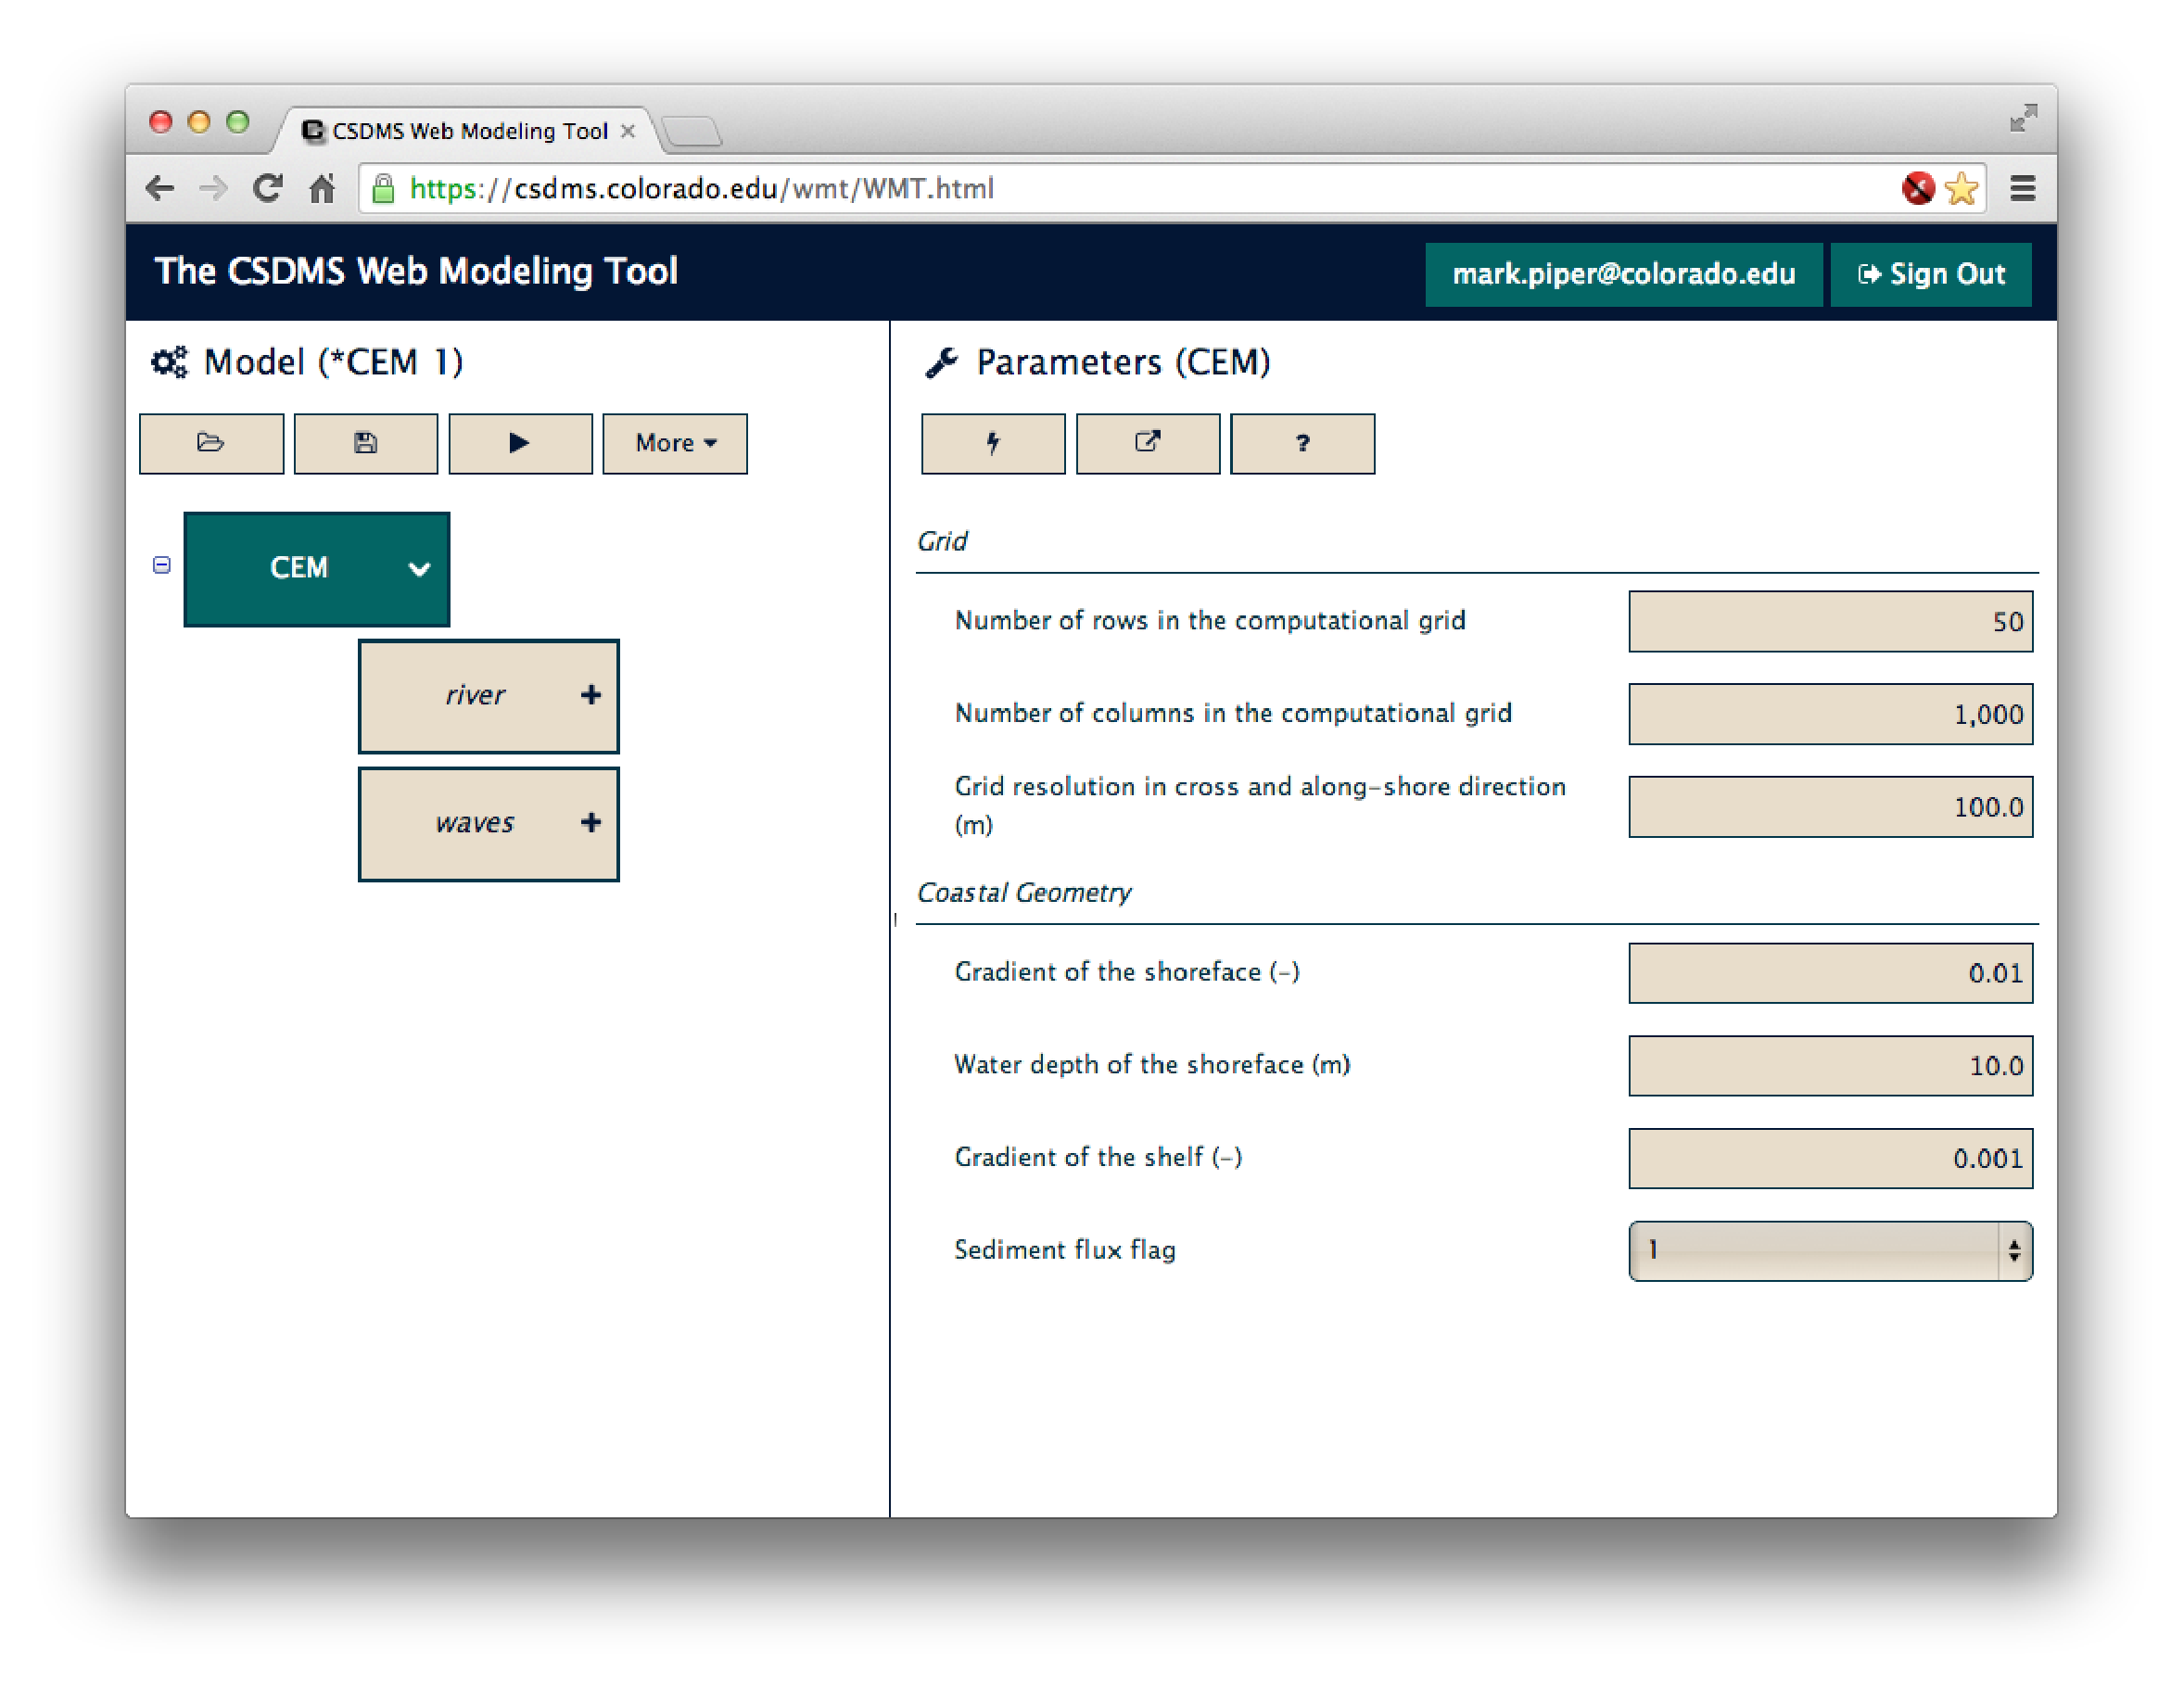
\includegraphics[scale=.25]{wmt.eps}
  \end{center}
  \label{fig:wmt_screenshot}
\end{figure}

\section{Acknowledgements}

The CSDMS Integration Facility operates under continuing grant 0621695 from the
US National Science Foundation.

\bibliographystyle{plain}

\bibliography{wssspe-citations}{}

\end{document}
